\newpage
\section{Grundlagen Kryptomining} \label{toc:grundlagenkryptomining}

\acused{SHA}

In diesem Kapitel werden die Grundlagen für das Verständnis des "`Kryptominings"' gelegt. Der Leser soll nach diesem Teil
ein Bild davon haben, was Mining ist und warum im Bereich Blockchain das Mining ein elementarer Prozess ist. Ferner soll
er in der Lage sein, den Grundaufbau eines unternehmensgeführten Rechenzentrums, das ausschließlich Mining betreibt, zu
verstehen. Um dies zu erreichen, wird im ersten Schritt in Kapitel \ref{toc:kryptowaehrungenundblockchain} eine kurze
Einführung zum Thema Blockchain gegeben und deren Grundaufbau beschrieben. Dort wird festgestellt, warum das Prinzip des
Minings eingeführt wurde und wofür es dient. Im Kapitel \ref{toc:miningundkonsensalgorithmen} wird vertieft auf den Prozess
des Minings eingegangen. Es wird die grundsätzliche Funktionsweise und die Notwendigkeit des Minings aufgezeigt. Nachdem
diese Grundlagen gelegt sind, wird die Funktionsweise eines Mining Rechenzentrums beschrieben. Das Verständnis von
Rechenzentren, die auf das Mining spezialisiert sind, ist wichtig für den Rest der Arbeit, da diese aus finanzieller
Sicht optimiert werden sollen. Dazu wird der Grundaufbau eines solchen Rechenzentrums der Genesis Group exemplarisch
beschrieben. Es wird gezeigt, welche \acp{KPI} dieser Rechenzentren wichtig sind. Diese werden verwendet, um die
Rechenzentren finanziell optimieren zu können. All das wird in Kapitel \ref{toc:miningrechenzentren} besprochen. Darauf
folgend wird dieses Wissen verwendet, um mögliche Ansatzpunkte für ein Business Intelligence System zu identifizieren
und am Ende der Arbeit einen beispielhaften Prozess zu modellieren.

\subsection{Grundlegende Technologien} \label{toc:technologie}

Das Konzept der Blockchain wurde erstmals im Jahr 2008 in einem Whitepaper anhand des Beispiels von Bitcoin beschrieben,
welches durch das Pseudonym Satoshi Nakamoto veröffentlicht worden ist.\footcite[Vgl.][]{nakamoto2008bitcoin} Es
beschäftigen sich inzwischen viele Unternehmen und Start-Ups in den verschiedensten Branchen mit Blockchain basierten
Systemen, wie beispielsweise in der Finanzbranche, im Informationssektor, aber auch im Gesundheits- und
Verkehrssektor.\footcite[Vgl.][Kap. 4.1]{friedlmaier2018disrupting} Ein anderer Zweig, der durch die Einführung von
Kryptowährungen entstanden ist, sind Unternehmen, die sich auf das Mining von Kryptowährungen spezialisiert haben. Um die
technischen Grundlagen für diesen Business Case zu verstehen, wird in den folgenden beiden Unterkapiteln beschrieben, was
eine Blockchain ist und welche Eigenschaften das Mining nötig macht. Wie Mining technologisch realisiert wird und warum
es eine Möglichkeit bietet, Geld zu verdienen, wird in Kapitel \ref{toc:miningundkonsensalgorithmen} beschrieben.

\subsubsection{Begriffsklärung Blockchain} \label{toc:kryptowaehrungenundblockchain}

Eine Blockchain ist, wie der Name übersetzt bedeutet, eine Kette aus Blöcken. Durch die Anwendung kryptographischer
Verfahren werden Daten auf einer Blockchain nachträglich unveränderlich gespeichert, was diese Technologie für viele
Anwendungen attraktiv machen kann.\footcite[Vgl.][S. 1]{friedlmaier2018disrupting} Die atomare Einheit einer Blockchain
ist ein einzelner Block. Dieser besteht im Fall von Bitcoin aus zwei verschiedenen Teilen: aus einer Liste von Transaktionen
sowie dem sogenannten "`Blockheader"', der die wichtigsten Metainformationen und Eigenschaften des Blocks
enthält.\footcite[Vgl.][S. 48]{bhaskar2015bitcoin}\footcite[Vgl.][S. 4]{nakamoto2008bitcoin}

\begin{figure}[H]
    \caption{Aufbau eines einzelnen Blocks}
    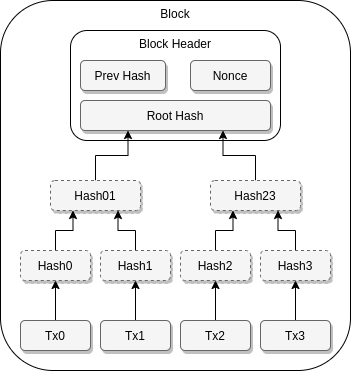
\includegraphics[width=0.4\textwidth]{blockstructure}
    \label{figure:blockstructure}
    \\
    \cite[Quelle: In Anlehnung an][S. 4]{nakamoto2008bitcoin}
\end{figure}

Im Folgenden sind die für das Verständnis elementaren Parameter aufgelistet, die in einem Blockheader zu finden
sind (Vgl. Abb. \ref{figure:blockstructure}):
\begin{itemize}
    \item \textbf{Previous block hash: }Da die Blöcke zu einer logischen Kette arrangiert werden, muss es eine
    Möglichkeit geben, die Reihenfolge der geschriebenen Blöcke zu identifizieren. Dies wird ähnlich zu einer
    verketteten Liste dadurch erreicht, dass aus dem Blockheader des vorhergehenden Blocks durch die Anwendung der \ac{SHA}256
    Hashfunktion ein Hash errechnet wird und dieser in das Feld "`Previous block hash"' eingetragen
    wird.\footcite[Vgl.][S. 4]{nakamoto2008bitcoin} Dadurch wird erreicht,
    dass die Reihenfolge der Blocks in der Blockchain wohldefiniert zurück bis zum ersten Block
    ("`Genesis Block"')\footcite[Vgl.][Abb. 3.2]{bhaskar2015bitcoin} nachvollziehbar ist (Vgl. Abb. \ref{figure:blockchainstructure}).
    Eine nachträgliche     Änderung eines Blocks wird die Kette brechen lassen, da sich dadurch der Hashwert des
    verfälschten Blocks ändern wird.
    \item \textbf{Merkle Root: }In dieses Feld wird das Ergebnis des Merkle Baums eingetragen, der aus allen Transaktionen
    errechnet wird.\footcite[Vgl.][S. 4]{nakamoto2008bitcoin} Auch dies ist ein Hashwert. Dazu wird ein Hashwert aus
    jeder einzelnen Transaktion gebildet und über einen Binärbaum zu einem Hashwert zusammengeführt. Dieser Wert nennt
    sich "`Merkle Root"' (Vgl. Abb. \ref{figure:blockstructure}). Dadurch lässt sich die Integrität jeder Transaktion,
    die sich in diesem Block befindet, überprüfen. Eine nachträgliche Änderung ist nicht mehr möglich, da in diesem
    Fall sich der Hashwert der Merkle Root im Blockheader und damit der resultierende Hash des Blockheaders ändern würde.
    Folglich bräche die Kette in diesem Fall und die Blockchain wäre zerstört.
    \item \textbf{Nonce: }Dies ist eine zufällige Nummer, die dafür verwendet wird, einen Hash des Blockheaders zu erzeugen,
    der bestimmten Rahmenbedingungen unterliegt.\footcite[Vgl.][S. 745]{mukhopadhyay2016brief}\footcite[Vgl.][S. 136]{courtois2014optimizing}
    Diesen Wert zu erraten und zu verifizieren wird Mining genannt.\footcite[Vgl.][S. 50f]{bhaskar2015bitcoin}\footcite[Vgl.][S. 24]{han2019demystifying}
    Wie dieser Wert gefunden wird und welchen Regeln er zu gehorchen hat, wird in Kapitel \ref{toc:miningundkonsensalgorithmen}
    beschrieben.
\end{itemize}

\begin{figure}[H]
    \caption{Schematischer Aufbau der Blockchain}
    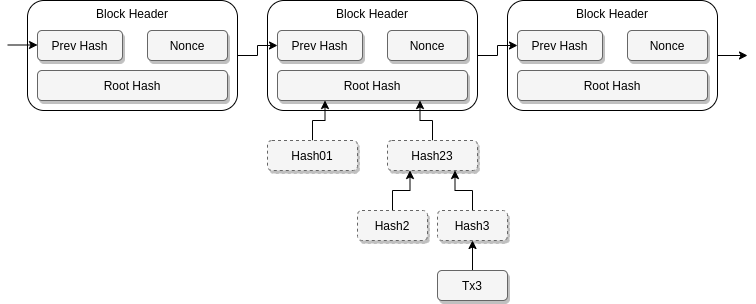
\includegraphics[width=0.8\textwidth]{blockchainstructure}
    \label{figure:blockchainstructure}
    \\
    \cite[Quelle: In Anlehnung an][S. 5]{nakamoto2008bitcoin}
\end{figure}

Der Rest des Blocks, der im Falle von Bitcoin auf die Größe von 1MB beschränkt ist, wird mit den dementsprechenden
Transaktionen gefüllt, die für die Errechnung der Merkle Root verwendet worden sind.\footcite[Vgl.][S. 746]{mukhopadhyay2016brief}
Generell können beliebige Daten auf einer Blockchain gespeichert werden. Dabei gibt es keine Beschränkungen, dass
es sich um Transaktionsdaten eine Währung handeln muss.

Nun exisitieren noch zwei Möglichkeiten, die Daten auf einer Blockchain zu verändern bzw. zu löschen. Der eine Fall
ist die manuelle Löschung der Blockchain. Um dies zu verhindern, ist eine Blockchain dezentral auf vielen Geräten
gespeichert.\footcite[Vgl.][S. 46]{bhaskar2015bitcoin} Jedes dieser Geräte beinhaltet eine aktuelle und korrekte Kopie
der Blockchain mit all ihren Daten. Ein solches Gerät wird "`Node"' genannt. Jede Person weltweit kann im Falle von
Bitcoin einen Node betreiben, da die Daten der Bitcoin Blockchain öffentlich einsehbar sind und es daher eine
sogenannte "`permissionless Blockchain"' ist.\footcite[Vgl.][S. 132]{courtois2014optimizing} Falls nun ein Teilnehmer
seinen Node löscht oder dieser einfach nur ausfällt, ist durch die dezentrale Replizierung die Blockchain weiterhin
verfügbar und nicht gelöscht.

Der andere Fall ist die Änderung eines Blocks und eine darauffolgende komplette Neuerrechnung aller Hashwerte dieser
Blockchain, womit wieder eine neue korrekte Blockchain daraus resultieren würde. Diese würde allerdings gefälschte Daten
beinhalten. Um dies zu verhindern, ist das Mining eingeführt worden, das nichts anderes als ein Ratespiel ist, um den
richtigen Wert der obig beschriebenen "`Nonce"' zu finden. Dieses Prinzip nennt sich \ac{PoW} und wird im nächsten Kapitel
genau beschrieben.\footcite[Vgl.][S. 3]{nakamoto2008bitcoin}

Zusammenfassend ist feststellbar, dass eine Blockchain aufgrund ihrer starken Anwendung kryptographischer Verfahren und
ihrer Dezentralität ausgesprochen sicher gegenüber der Fälschung und Löschung von Daten ist. Der erste naheliegende
Use-Case war dementsprechend die Anwendung der Blockchain, um eine digitale und dezentrale Währung einzuführen, wie es
Satoshi Nakamoto auch in seinem Whitepaper vorgeschlagen hat.\footcite[Vgl.][]{nakamoto2008bitcoin}

\subsubsection{Begriffsklärung Mining} \label{toc:miningundkonsensalgorithmen}

In diesem Kapitel wird sich aufbauend auf dem letzten Kapitel mit der Funktionsweise des Minings und der unterliegenden
Konsensalgorithmen beschäftigt. Dies ist für die weitere Arbeit wichtig, da das den prinzipiellen Aufbau von Mining
Rechenzentren begründet und auch während des Minings wichtige Parameter, wie die "`Difficulty"' eine Rolle spielen, die
für eine finanzielle Gesamteinschätzung eines Rechenzentrums einen Beitrag leisten.

Ausgehend von der Problematik, dass die Bitcoin Blockchain aus einem dezentralen peer-to-peer Netzwerk besteht, muss
sich die Frage gestellt werden, wie ein Konsens zwischen den Teilnehmern erzeugt wird und wie sichergestellt wird,
dass betrügerische Absichten unterbunden werden. Es wird die Frage gestellt, wie alle Teilnehmer zusammen einen gültigen
Konsens erreichen und damit die Blockchain vertrauenswürdig wird.\footcite[Vgl.][Abb. 3]{derks2018chaining}
Um diese Fragestellungen zu beantworten, wird sich mit möglichen Konsensalgorithmen beschäftigt und das Prinzip
des Minings anhand des \ac{PoW} Konsenses erläutert.

Der erste Konsensalgorithmus wurde im Bitcoin Whitepaper von Satoshi Nakamoto beschrieben und nennt sich
"`Proof-of-Work"'.\footcite[Vgl.][S. 3]{nakamoto2008bitcoin} Da dieser in Hinsicht auf den Energieverbrauch nicht
optimal ist, sind für andere Währungen andere Algorithmen, die deutlich energieeffizienter sind, erarbeitet
worden.\footcite[Vgl.][]{dwcom2021bitcoin} Das bekannteste Beispiel ist \ac{PoS} oder auch die Verwendung der
"`byzantinischen Fehlertoleranz"', das auch als das "`Problem der byzantinischen Generäle"' über die Blockchain
Branche hinweg bekannt ist.\footcite[Vgl.][S. 2]{friedlmaier2018disrupting}\footcite[Vgl.][S. 746]{mukhopadhyay2016brief}
Da allerdings nur für Proof-of-Work große Rechenleistungen benötigt werden, wird sich im Folgenden auf diesen Algorithmus
anhand des Beispiels von Bitcoin beschränkt.

Der Vorgang des Minings durch Proof-of-Work lässt sich in die folgenden Schritte
unterteilen:\footcite[Vgl.][S. 3]{nakamoto2008bitcoin}\footcite[Vgl.][S. 51]{li2019blockchain}

\begin{enumerate}
    \item Neue Transaktionen werden zu allen Nodes im Netzwerk gesendet. Diese werden im sogenannten "`Mempool"',
    einem Zwischenspeicher für noch nicht bestätigte Transaktionen abgelegt und für den Miningprozess vorgehalten.
    \item Transaktionen werden durch die Nodes in einen Block verpackt. Die Transaktionen mit den höchsten Gebühren,
    die vom Auftraggeber frei gewählt werden können, werden bevorzugt aus dem Mempool zu einem Block
    zusammengeführt.\footcite[Vgl.][S. 53]{bhaskar2015bitcoin} Die Summe der Transaktionskosten des Blocks wird dem Miner
    zugeschrieben, sobald dieser einen gültigen Block findet.\footcite[Vgl.][S. 4]{nakamoto2008bitcoin}
    \item Die Mining Hardware errechnet einen gültigen Proof-of-Work für diesen Block, den die Nodes der Hardware zur
    Verfügung stellen. Dies ist der eigentlich rechenintensive Prozess. Grundlegend ist dieser Vorgang nichts
    anderes als ein Brute-Forcing von Hashwerten.\footcite[Vgl.][S. 747]{mukhopadhyay2016brief} Nur auf diesem Weg ist
    es möglich, einen korrekten Zielhashwert zu errechnen, da Hashfunktionen surjektiv sind. Durch die sogenannte
    "`Difficulty"' wird festgelegt, mit wie vielen Nullen der resultierende Hash beginnen
    soll.\footcite[Vgl.][S. 57]{bhaskar2015bitcoin} Um einen passenden Hash zu finden, wird die Nonce variiert und
    für jeden Wert der Nonce der Hashwert des Blocks berechnet und verifziert, ob dieser den Anforderungen, die
    durch die Difficulty vorgegeben ist, genügt. Im Durchschnitt sollte dieser Vorgang circa zehn Minuten in Anspruch
    nehmen.\footcite[Vgl.][S. 748]{mukhopadhyay2016brief} Die relevante Leistungmetrik der Mining Hardware wird daher
    Hashrate genannt.\footcite[Vgl.][S. 49]{bhaskar2015bitcoin} Diese beschreibt, wie viele Hashwerte ein Gerät innerhalb
    einer Sekunde errechnen kann. Falls die gesamte Hashrate im Bitcoin Netzwerk steigt, steigt auch die
    Wahrscheinlichkeit, dass ein gültiger Proof-of-Work in kürzer als zehn Minuten gefunden werden kann. Daher wird die
    Difficulty alle 2.016 Blocks angepasst, sodass es bei einer höheren Gesamthashrate des Netzwerks durch die Variation
    der beginnenden Nullen leichter oder schwieriger wird, einen gültigen Proof-of-Work zu finden (Vgl.
    Abb. \ref{figure:evolutiondifficulty}).\footcite[Vgl.][S. 57]{bhaskar2015bitcoin} Da die Erstellung der Blöcke
    viel rechnerische Arbeit kostet, haben nun einzelne Betrüger keine Mögtlichkeit, die Blockchain zu manipulieren,
    solange die Mehrheit der Teilnehmer am Mining ehrlich ist. 
    \item Wenn ein Proof-of-Work gefunden ist, wird dieser an alle Nodes im Bitcoin Netzwerk
    gesendet.\footcite[Vgl.][S. 3f]{nakamoto2008bitcoin} Dazu formt der zur Mining Hardware verbundene Node aus der
    gültigen gefundenen Nonce und allen weiteren Informationen einen gültigen neuen Block und sendet diesen an alle
    Nodes im Bitcoin Netzwerk.
    \item Dieser wird nun von den verbleibenden Nodes überprüft. Die Verifizierung ist erfolgreich, sobald die Mehrzahl
    an Nodes den Block akzeptiert und mit dem Bau eines neuen Blocks begonnen wird, wobei der Hashwert des gefundenen
    Blocks als Previous Hash für den neuen Block verwendet wird.\footcite[Vgl.][S. 3f]{nakamoto2008bitcoin}
    Der Betreiber der Mining Hardware erhält als Belohnung die Summe aller Transaktionengebühren des Blocks und
    zusätzlich einen Festbetrag, der momentan bei 6,25 \ac{BTC} pro Block
    liegt.\footcite[Vgl.][S. 4]{nakamoto2008bitcoin}\footcite[Vgl.][]{btcecho2021halving}\footcite[Vgl.][S. 59]{taylor2017evolution}
    Die 6,25 \ac{BTC} nennen sich "`Block Reward"'. Dieser betrug anfangs 50 \ac{BTC} und wird alle 210.000 Blöcke um
    die Hälfte reduziert.\footcite[Vgl.][S. 58]{taylor2017evolution} Dadurch wird das Bitcoin Netzwerk mit neuer und
    frischer Währung versorgt. Folgend beginnt der Prozess des Minings wieder von vorne.
\end{enumerate}

\begin{figure}[H]
    \caption{Entwicklung der Difficulty von Bitcoin abhängig von der verwendeten Hardware und Fertigungsgröße}
    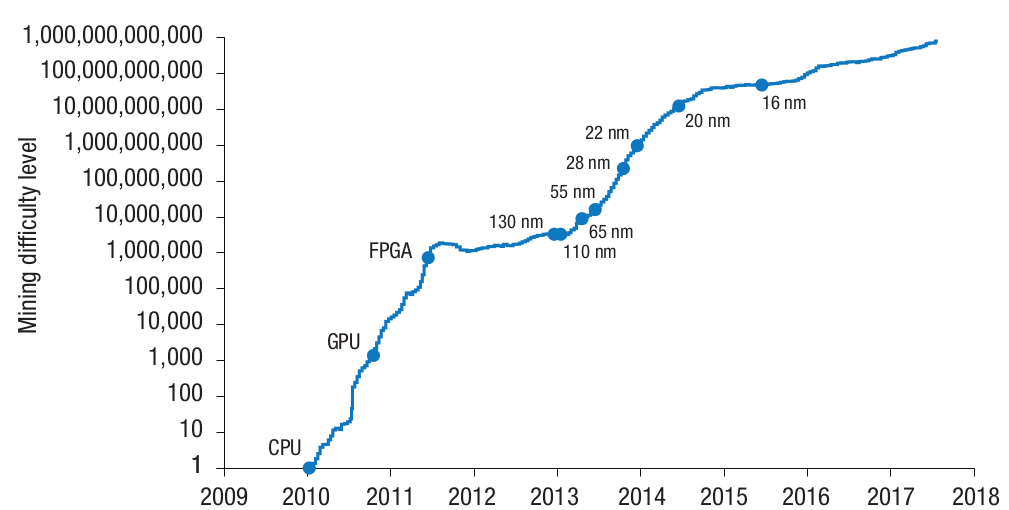
\includegraphics[width=0.8\textwidth]{evolutiondifficulty}
    \label{figure:evolutiondifficulty}
    \\
    \cite[Quelle: ][Abb. 1b]{taylor2017evolution}
\end{figure}

Prinzipiell ist die Wahrscheinlichkeit, einen Block als Erster erfolgreich zu finden umso höher, je höher der eigene
Anteil an der gesamten Hashrate des Netzwerks ist. Aus diesem Grund versuchen Betreiber von Mining Hardware so viel
Leistung wie möglich dem Netzwerk zur Verfügung zu stellen, um möglichst hohe Auszahlungen zu erhalten. Der Betrieb
findet in Abhängigkeit zu den Kosten für eine solche Infrastruktur statt, was in Kapitel
\ref{toc:kennzahlenundeinflussfaktoren} näher erörtert wird.

Grundsätzlich kann jeder am Mining teilnehmen. Es gibt momentan drei Modelle, wie Mining betrieben werden
kann:\footcite[Vgl.][S. 53, S. 57ff]{bhaskar2015bitcoin}
\begin{itemize}
    \item \textbf{Solo Mining: }Dies beschreibt die klassische Methode, in welcher Teilnehmer ihre eigene Hardware
    verwenden und Mining betreiben. Diese bekommen nach einem erfolgreichen Proof-of-Work den gesamten Ertrag eines Blocks.
    \item \textbf{Mining Pools: }Bei Mining Pools wird die Hashrate vieler Miner zusammengeführt. Durch die Bündelung
    der Hashrate wird die Wahrscheinlichkeit, einen gültigen Block zu finden, gesteigert. Die Auszahlung ist in diesem
    Verfahren nicht der Gesamtertrag des Blocks, sondern der prozentuale Anteil der Leistung, die dem Mining Pool zur
    Verfügung gestellt wird. Durch die Beteiligung werden die einzelnen Erträge zwar geringer jedoch gleichmäßiger
    ausfallen. Dadurch wird dem Risiko entgangen, als Solo Miner lange keinen gültigen Proof-of-Work zu finden
    (s. Abb. \ref{figure:valuechaindatacenter}).\footcite[Vgl.][S. 58ff]{bhaskar2015bitcoin}\footcite[Vgl.][S. 327]{derks2018chaining}
    \item \textbf{Mining Contracts: }Die dritte Möglichkeit ist die Miete von Mining Hardware oder der Kauf von
    Hashrate. \footcite[Vgl.][S. 58ff]{bhaskar2015bitcoin} Der Erlös aus dem Mining wird der Person nach Abzug der
    Vertragsgebühren überwiesen. Folglich muss die Person keine eigene Hardware betreiben und kann dies professionellen
    Unternehmen überlassen, die dies deutlich effizienter als Privatpersonen durchführen können. Solch ein Produkt bietet die
    Genesis Group an.
\end{itemize}

\subsection{Mining Rechenzentren} \label{toc:miningrechenzentren}

Das Mining von Bitcoins hat sich seit der Einführung 2009 stark verändert. Damals wurde begonnen, Hashes auf
normalen \acp{CPU} zu berechnen.\footcite[Vgl.][S. 97f]{xie2018extreme}\footcite[Vgl.][S. 62]{taylor2017evolution}
Wie bereits in Kapitel \ref{toc:miningundkonsensalgorithmen} erklärt, steigt die Wahrscheinlichkeit, einen Block
erfolgreich mittels Proof-of-Work zu finden, mit der anteiligen Hashrate an der gesamten Netzwerkhashrate.
Dementsprechend wollen die Betreiber von Mining Hardware die Effizienz durch die Reduzierung der Kosten pro
errechnetem Hash steigern. Durch dieses Bestreben ist die zweite Generation der Mining Hardware auf Basis von
\acp{GPU} entwickelt worden.\footcite[Vgl.][S. 98]{xie2018extreme}\footcite[Vgl.][S. 62]{taylor2017evolution}
Durch die Entwicklung der Netzwerkhashrate von Bitcoin ist folgend die Hardware der dritten Generation auf der
Grundlage von \acp{FPGA} entwickelt worden.\footcite[Vgl.][S. 98]{xie2018extreme}\footcite[Vgl.][S. 62f]{taylor2017evolution}
Der Hardwaretyp der vierten Generation ist bis heute im Einsatz und basiert auf
\acp{ASIC}.\footcite[Vgl.][S. 98f]{xie2018extreme}\footcite[Vgl.][S. 15]{gai2020blockchain} Diese Geräte sind
durch das Hardwarelayout darauf spezialisiert, hocheffizient Hashes zu berechnen.\footcite[Vgl.][S. 15]{gai2020blockchain}
Auf der anderen Seite sind diese Chips nicht in der Lage, andere Dinge effizient zu berechnen und sind daher nur für diesen
spezifischen Zweck entwickelt worden. Allerdings gab es nicht nur das Bestreben nach höherer Effizienz, sondern auch
nach einer Skalierung der Mining Hardware. Um die Erträge aus dem Mining zu maximieren, wurden diese beiden Treiber
kombiniert. Dies führte zum Bau von hochspezialisierten, ASIC basierten Rechenzentren, die alleinig dem Bitcoin Mining
gewidmet sind.\footcite[Vgl.][S. 97]{xie2018extreme} Mehrere solche Rechenzentren betreibt die Genesis Group. Diese werden
im Folgenden exemplarisch beschrieben und deren Kosten- und Wertstruktur analysiert.

\subsubsection{Aufbau und Funktionsweise} \label{toc:aufbauundfunktionsweise}

In diesem Kapitel wird beschrieben, wie ein Rechenzentrum, das auf Bitcoin Mining spezialisiert ist, aufgebaut ist
und wie dieses Mining betreibt.

Zentraler Bestandteil eines Mining Rechenzentrums ist die Mining Hardware.\footcite[Vgl.][S. 327]{derks2018chaining}
Die Anzahl der Geräte, die in einem solchen Rechenzentrum betrieben werden, ist grundsätzlich nur durch äußere Faktoren
wie Platzangebot und Stromversorgung limitiert. In dem Paper "`Extreme Datacenter Specialization for Planet-Scale
Computing: ASIC Clouds"' wird beschrieben, dass die Geräte meist in Serverschränken untergebracht
werden.\footcite[Vgl.][Abb. 5]{xie2018extreme} Dies bei Mining Rechenzentren in der Regel nicht der Fall,
da der Großteil der Hardware nicht im 19 Zoll Formfaktor gebaut wird. Stattdessen werden passende Schwerlastregale
verwendet, die in Reihe aufgestellt werden. Viele solcher Reihen bilden das Rechenzentrum an
sich.\footcite[Vgl.][]{appendix:layoutkardok}

Da die Mining Hardware viel Strom verbraucht, muss besonderer Wert auf die Stromversorgung gelegt
werden.\footcite[Vgl.][S. 327]{derks2018chaining} Der nötige Strom wird von externen Energieunternehmen bezogen. Die
Umspannwerke und nötigen Transformatoranlagen sind auf dem Außengelände des Rechenzentrums bzw. sehr nah gelegen
aufgebaut und stellen eine stabile Stromversorgung sicher. Innerhalb des Rechenzentrums sind Starkstromunterverteiler
errichtet, die letztendlich für die Versorgung der einzelnen Geräte benötigt werden. Eines der aktuellen Modelle,
der S19 Pro Miner von Bitmain, verbraucht pro Gerät im Durchschnitt 3,25kW.\footcite[Vgl.][]{s19pro2021consumption}
Ausgehend von der Annahme, dass in einem Rechenzentrum circa 12.000 Geräte aufgestellt sind, ergibt sich ein gesamter
Stromverbrauch von 39,0MW für die Mining Hardware.

Damit die Miner stabil betrieben werden können, muss die Abwärme der Geräte effizient abtransportiert werden. Dazu
wird ein grundlegender Aufbau identisch zu einem gewöhnlichen Rechenzentrum bestehend aus Heiß- und Kaltgang verwendet.
Durch Lüfter wird kalte Luft von außen in das Rechenzentrum transportiert. Diese erwärmt sich, während sie durch die
Mining Hardware fließt, und wird durch den Heißgang abtransportiert.\footcite[Vgl.][]{appendix:layoutkardok} Die
Stromkosten für die Kühlung machen einen erheblichen Anteil der Stromkosten eines Mining Rechenzentrums aus.

Damit die Mining Hardware mit den Blockchain Nodes kommunizieren kann, ist neben der Stromversorgung auch eine
Netzwerkinfrastruktur notwendig. Diese ist so konzipiert, dass jedes Geräte mit dem Internet und damit auch den Nodes
kommunizieren kann. Aufgrund der Anforderungen an die Bandbreite des internen Netzwerkes sind die zentralen
Komponenten mit einem Durchsatz von 10$\frac{Gbit}{s}$ dimensioniert. Für die Peripherie genügt eine Datenmenge
von 1$\frac{Gbit}{s}$.\footcite[Vgl.][]{appendix:networktopology} Um die Bandbreite in das Internet möglichst
gering zu halten, wird die Mining Hardware mit einem Mining Proxy verbunden, der auf einem internen Server
installiert ist und die Verbindung zum Bitcoin Netzwerk und dem verwendeten Mining Pool
herstellt.\footcite[Vgl.][]{appendix:miningproxy} Der Vorteil liegt darin, dass zu einem externen Mining Pool
nur noch eine Verbindung benötigt wird.

Schlussendlich ist auf weiteren internen Servern eine Steuerungs- und Überwachungssoftware für die Mining Hardware
installiert. Durch diese Software wird eine große Anzahl von Mining Geräten gesteuert und
überwacht.\footnote{https://www.genesis-mining.com/hexa} Die gewonnenen Daten aus der Überwachung können sehr
interessant für die Verwendung innerhalb von Business Intelligence Prozessen sein. Diese Evaluation geschieht
in Kapitel \ref{toc:ansatzmoeglichkeitenfuerbusinessintelligence}.

\subsubsection{Finanzielle Betrachtungen} \label{toc:kennzahlenundeinflussfaktoren}

In diesem Teil wird nun beschrieben, welche finanziellen und nicht-finanziellen Einflussfaktoren bei einem
Rechenzentrum, das sich auf Mining spezialisiert hat, existieren. Dazu wird sich bei finanziellen Aspekten auf interne
Dokumentationen gestützt. Diese werden zusätzlich kategorisiert, ob es sich um \ac{CapEx} oder \ac{OpEx} Posten und
ob es sich um variable oder fixe Kosten handelt. Weiterhin werden Faktoren erläutert, die die Einnahmen des Rechenzentrums
optimieren können und wie die Rentabilität gemessen werden kann (\acp{KPI}). Richtung Ende werden Einflussfaktoren
gelistet, die nicht-finanzieller oder nicht-technischer Natur sind und momentan daher grundsätzlich nur in einem geringen
Detaillierungsgrad in Betracht gezogen werden können. Sprungfixe Kosten werden in diesem Teil nicht verwendet, da die
zugrundeliegenden Berechnungen und Abschätzungen diese auch nicht als Kostensorte berücksichtigen.


Die Kosten eines Rechenzentrums werden im ersten Schritt grundlegend in \ac{CapEx} und \ac{OpEx}
unterteilt.\footcite[Vgl.][]{appendix:capex}\footcite[Vgl.][]{appendix:opex} \ac{CapEx} beschreibt dabei die initialen
Ausgaben, die für den Aufbau eines Datencenters getätigt werden müssen. \ac{OpEx} beschreibt die Sorte von Kosten, die permanent
während des Betriebs entstehen. Beide Posten werden zusätzlich in fixe oder variable Kosten unterteilt, die abhängig
von der Zahl der Miner sind, die vor Ort installiert wird.

\begin{figure}[H]
    \caption{Kostenstruktur eines Mining Rechenzentrums}
    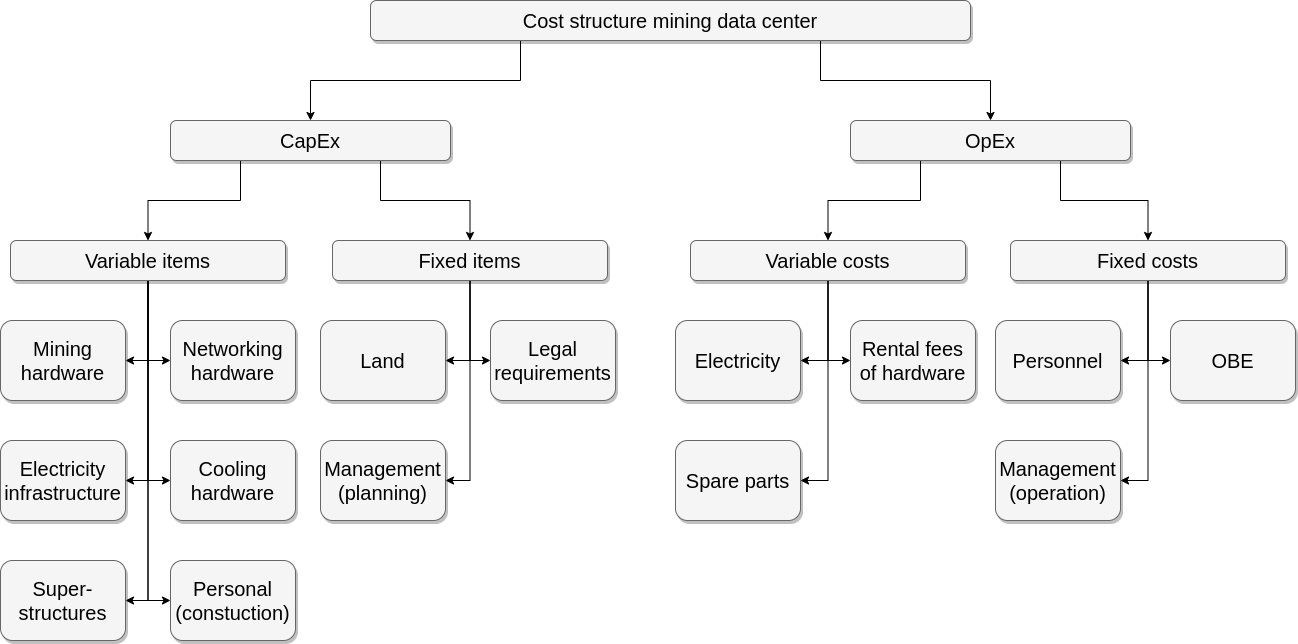
\includegraphics[width=\textwidth]{valuestructurenordics}
    \label{figure:valuestructurenordics}
\end{figure}

Diese Aufteilung ist in Abb. \ref{figure:valuestructurenordics} zu finden. Die folgenden Posten sind für den Aufbau
eines Rechenzentrums relevant:\footcite[Vgl.][]{appendix:capex}
\begin{itemize}
    \item \textbf{Mining Hardware: }Mit diesem Posten ist die eigentliche spezielle Hardware gemeint, die für das
    Bitcoin Mining benötigt wird (s. Ziffer 2 in Abb. \ref{figure:valuechaindatacenter}). Der \ac{KPI}, der die
    Effektivität des Geräts misst, ist die Höhe der durchschnittlichen Auszahlungen durch das Mining. Diese bewegt
    sich bei aktuellen Modellen, wie dem Antminer S19Pro, im ungünstigsten Fall bei $0,06\ USD / \frac{TH}{s} / day$, d.h.
    \ac{USD} pro Hashrate pro Tag.\footcite[Vgl.][]{appendix:worstcasescenario} Im wahrscheinlichsten Szenario liegt
    es bei $0,09\ USD / \frac{TH}{s} / day$\footcite[Vgl.][]{appendix:mostprobablescenario} und im optimalen Szenario
    bei $0,27\ USD / \frac{TH}{s} / day$.\footcite[Vgl.][]{appendix:optimalscenario} Die Identifikation des korrekten
    Szenarios ist anhand der Difficulty des Bitcoin Minings, der gesamten Netzwerk Hashrate und anhand des Marktwerts
    eines Bitcoin möglich, was weitere \acp{KPI} beim Betrieb eines Rechenzentrums sind. Da der Marktwert ausgesprochen
    volatil ist, ist es schwer eine genaue Vorhersage zu treffen.\footcite[Vgl.][S. 325]{badertscher2017bitcoin} Zusätzlich
    sind in diesem Teil die Ausfalldauer und die Gebühren für den Mining Pool pauschal mit
    einberechnet.\footcite[Vgl.][]{appendix:s19proassumptions} Die Effektivität der Mining Hardware wird folgendermaßen
    berechnet:
    \begin{equation}
        \RM = \frac{\DP}{\THr}\cdot(1-\PF)\cdot\UT\cdot\ER
    \end{equation}
    In dieser Formel werden die täglich erwarteten Auszahlungen (\DP) pro Hashrate (\THr) berechnet. Das Resultat wird
    dabei durch Uptime der Mining Hardware (\UT), Gebühren (\PF) und dem Tauschkurs von \ac{USD} und \ac{BTC} korrigiert.

    Bei dieser Rechnung ist nicht der Strompreis direkt aufgeführt. Diese Größe wird über den Stromverbrauch der Geräte
    errechnet. Verbesserungen in der Firmware dieser Geräte können mit einem \ac{KPI} visualisiert werden, der sich
    "`Reference power effiency"' nennt. Dieser hat die Einheit $\frac{J}{TH}$ (Joule pro Terahash) und ist stark
    temperaturabhängig.\footcite[Vgl.][]{s19pro2021consumption}

    Der Posten der Mining Hardware ist variabel, da sich dieser proportional zur Anzahl der Miner verhält. Bei einem
    10MW Rechenzentrum wären dies circa 2.987 S19 Pro Miner\footcite[Vgl.][]{appendix:s19proassumptions} bei einem Gesamtpreis
    von circa 8.068.708 USD.\footcite[Vgl.][]{appendix:capex}
    \item \textbf{Netzwerk Hardware: }Damit die Mining Hardware mit der Blockchain kommunizieren kann, wird die Netzwerk
    Hardware benötigt. Unter diesen Posten fallen Switches, Router und Netzwerkkabel. Es wird dabei auf standartisierte
    Netzwerk Hardware zurückgegriffen, die günstig und in großen Stückzahlen verfügbar ist. Dieser Posten ist ebenfalls
    variabel, da sich mit steigender Anzahl von Mining Hardware auch die Anzahl und Länge der Netzwerkverkabelung und die Anzahl
    der Switches erhöht.\footcite[Vgl.][]{appendix:capex} Die Zahl der Router bleibt zwar konstant, stellt aber nur einen so
    geringen Anteil an diesem Posten dar, sodass dieser als variabel angesehen werden kann. Bei einem 10MW Rechenzentrum
    liegen die Kosten für diesen Posten bei circa 69.060 USD.\footcite[Vgl.][]{appendix:capex}
    \item \textbf{Infrastruktur Elektrizität: }Für den Betrieb der Mining Hardware ist ein Posten bei der Errichtung
    eines Mining Rechenzentrums die Energieversorgung. Bei diesem Posten ist vor allem die Verkabelung innerhalb des
    Rechenzentrums gemeint. Die Netzanbindung und die Starkstromtransformatoren werden in anderen Posten in die Rechnung
    mit einbezogen. Da  die Anzahl der Kabel und Verteiler innerhalb eines Rechenzentrums mit steigender Anzahl von Mining
    Geräten zunimmt, ist dies ein variabler Posten bei der Errichtung.\footcite[Vgl.][]{appendix:capex} Die Kosten belaufen
    sich auf circa 423.900 USD für ein Rechenzentrum mit einem Mining Stromverbrauch von 10MW.\footcite[Vgl.][]{appendix:capex}
    \item \textbf{Hardware Kühlung: }Wie in allen anderen Rechenzentren muss auch eine Kühlung vor Ort errichtet werden.
    Dabei handelt es sich hauptsächlich um Lüfter und Filter, die installiert werden müssen.
    Da die Anzahl der Kühlungsgeräte mit der Anzahl von installierten Mining Geräten skaliert, ist dies ein variabler Posten.
    Bei der Energieversorgung stellt die Kühlung einen konstanten prozentualen Anteil an dem Gesamtverbrauch dar.
    Dieser Wert ist primär vom Klima (Temperatur) vor Ort anhängig, welches daher einen \ac{KPI} darstellt. Dieser Posten
    hat circa die Höhe von 908.350 USD für ein 10MW Mining Rechenzentrum.\footcite[Vgl.][]{appendix:capex}
    \item \textbf{Aufbauten: }Dabei handelt es sich primär um Schwerlastregale, die für die Aufstellung der Miner verwendet
    werden. Auch sind dort weitere Posten enthalten, die den Aufbau und die Anpassung des Mining Rechenzentrums betreffen. Da sich
    diese Anpassungen und die Anzahl der Schwerlastregale mit steigender Anzahl der Mining Hardware erhöhen, wird dieser
    Teil als ein variabler Posten betrachtet. Bei einem 10MW Rechenzentrum beläuft sich dieser Teil auf circa 284.850
    USD.\footcite[Vgl.][]{appendix:capex}
    \item \textbf{Personal (Aufbau): }Für den Aufbau eines Rechenzentrums wird initial Personal benötigt. Dabei handelt es
    sich vor allem um Fachpersonal im Bereich IT und Elektrik, das für den Aufbau angestellt wird. Dieser Teil wird mit circa
    297.321 \ac{USD} in die Berechnung der \ac{CapEx} mit einbezogen.\footcite[Vgl.][]{appendix:capex} Es ist ein variabler
    Posten, denn je größer ein Rechenzentrum wird desto mehr Personal wird für einen Aufbau benötigt.\footcite[Vgl.][]{appendix:capex}
    \item \textbf{Land: }In diesem Punkt wird das Land und die Immobilie für ein Mining Rechenzentrum mit einbezogen. Die
    benötigten finanziellen Mittel sind stark von dem Ort abhängig, an dem ein Rechenzentrum errichtet werden soll. In der
    Beispielrechnung für das 10MW Rechenzentrum, das auch bei den letzten Punkten verwendet wurde, war die Höhe der Kosten
    für diesen Posten bei circa 1.223.691 \ac{USD}.\footcite[Vgl.][]{appendix:capex} In diesem Fall wird dieser Posten nicht
    als variable Kosten benannt, obwohl dies naheliegend sein könnte. Aus diesem Grund handelt es sich um einen fixen Posten,
    da ein Grundstück im Verkauf eine festgelegte Größe hat. Es ist nicht möglich, je nach Bedarf ein Grundstück zu verkleinern
    oder zu vergrößern. Deshalb zählt dies zu den fixen Posten.\footcite[Vgl.][]{appendix:capex}
    \item \textbf{Gesetzliche Anforderungen: }Je nach Land, in dem Mining Rechenzentren errichtet werden sollen, sind
    verschiedene gesetzliche Anforderungen zu berücksichtigen. Dabei handelt es sich vor allem um Voraussetzungen, die den
    Betrieb eines solchen Rechenzentrums und die Beschäftigung von Personal möglich machen. Das lokale Steuerrecht ist im
    Besonderen zu berücksichtigen. Diese Ausgaben, die zu großen Teilen aus Anwaltskosten bestehen, sind bereits vor der
    Errichtung eines Rechenzentrums zu beachten und treten einmalig auf. Sie belaufen sich auf 1.735.295 \ac{USD}, wenn
    das Beispiel des 10MW Rechenzentrums zu Grunde gelegt wird.\footcite[Vgl.][]{appendix:capex}
    \item \textbf{Management (Planung): }Letztendlich werden unter \ac{CapEx} das initiale Management und die Kosten für
    das Projektmanagement kalkuliert. Das sind die Kosten für das Personal, die zentral solche Rechenzentren und die
    dazugehörigen Projekte planen. Für das beispielhafte Rechenzentrum beläuft sich dieser Posten auf circa
    631.880 USD.\footcite[Vgl.][]{appendix:capex}
\end{itemize}

Durch die Summation aller Werte der vorherigen Punkte ist feststellbar, dass ein Rechenzentrum, das eine Mining Kapazität
von 10MW aufweisen soll, circa 13.665.996 USD kostet.\footcite[Vgl.][]{appendix:summaryofinvestment} Die Verteilung der
beschriebenen einzelnen Posten ist in Abbildung \ref{figure:capexdistribution10mw} relativ zueinander anhand der Zahlen für
ein 10MW Rechenzentrum abgebildet.

\begin{figure}[H]
    \caption{CapEx Verteilung bei einem 10MW Rechenzentrum}
    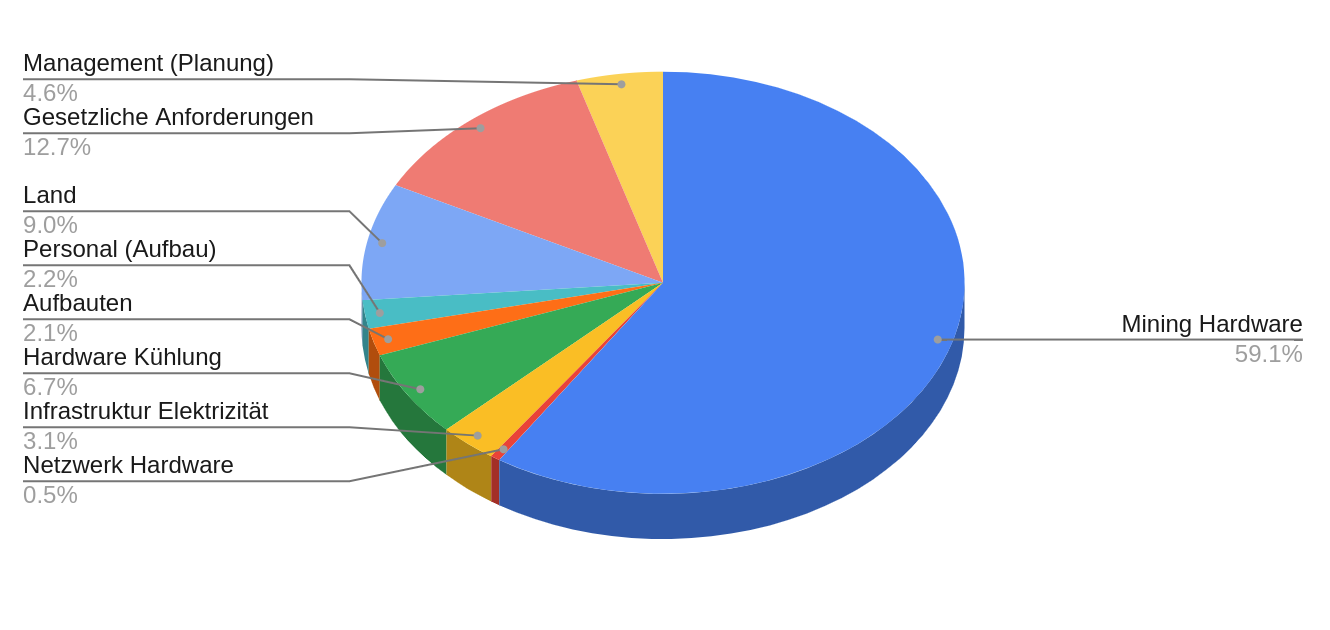
\includegraphics[width=0.7\textwidth]{capexdistribution10mw}
    \label{figure:capexdistribution10mw}
\end{figure}

Neben den Ausgaben, die initial bei einem Rechenzentrum beachtet werden müssen, sind auch die folgenden Kosten (\ac{OpEx}),
die während dem Betrieb entstehen, zu beachten:\footcite[Vgl.][]{appendix:opex}
\begin{itemize}
    \item \textbf{Elektrizität: }Dieser Teil beschreibt die Kosten, die durch den Verbrauch von Elektrizität erzeugt werden.
    Dieser Parameter ist ein zentraler Bestandteil bei der Betrachtung von \acp{KPI} eines Kryptomining Rechenzentrums
    (s. Abb. \ref{figure:valuechaindatacenter}).\footcite[Vgl.][S. 327]{derks2018chaining} Da ein Mining Rechenzentrum
    Großabnehmer bei Energieversorgern ist, unterliegen die Preise einer Schwankung, die von dem Anbieter vorgegeben
    ist.\footcite[Vgl.][]{appendix:opex} Dieser Posten gehört zu den variablen Kosten, da mit ansteigender Zahl von Geräten
    für Mining und Kühlung der Stromverbrauch steigt. Die jährlichen Kosten für ein 10MW Rechenzentrum betragen bei einem
    Grundpreis von $0.0357 \frac{USD}{kWh}$ circa 3.038.313 USD.\footcite[Vgl.][]{appendix:opex}
    \item \textbf{Leihgebühren Hardware: }Hierbei werden Geräte geführt, die geliehen sind und daher in regelmäßigen
    Zeitabständen bezahlt werden müssen. Im Falle der Genesis Group sind dies die Hauptverteiler und Transformatoren
    eines Rechenzentrums, die eine Kapazität größer 1MW haben. Da diese Geräte im Kauf sehr teuer sind, werden sie von
    den Energieversorgern geliehen. Die jährlichen Kosten für einen solchen Leih sind bei 10MW circa 170.280 USD
    und sind variabler Natur.\footcite[Vgl.][]{appendix:opex}
    \item \textbf{Ersatzteile: }Um Defekte jeglicher Hardware vor Ort reparieren zu können, findet sich der Posten der
    Ersatzteile in der Berechnung für den \ac{OpEx}.\footcite[Vgl.][S. 327]{derks2018chaining} Für diesen Teil stehen
    keine beispielhaften Zahlen zur Verfügung.
    \item \textbf{Personal: }Damit die Hardware repariert werden kann und der Betrieb des Rechenzentrums aufrecht erhalten
    werden kann, wird Personal permanent vor Ort benötigt. Dieser Posten beläuft sich in dem Beispiel auf circa
    31.282 USD pro Monat, kann sich aber von Land zu Land durchaus drastisch unterscheiden.\footcite[Vgl.][]{appendix:opex}
    Dieser Betrag ist unter den Fixkosten aufgeführt, da durch die anfängliche Größe des Rechenzentrums auch die Personalplanung
    klar ist. Es wird auch bei kleinen Erweiterungen kein weiteres Personal angestellt.\footcite[Vgl.][]{appendix:opex}
    \item \textbf{Management (Betrieb): }Für die Verwaltung des Rechenzentrums und das zentrale Projektmanagement wird
    außerdem eine weitere Pauschale von 6.289 USD pro Monat aufgerufen.\footcite[Vgl.][]{appendix:opex} Diese beschreibt
    die Verwaltungskosten von zentraler Seite aus.
    \item \textbf{\ac{BGA}: }In diesem Bereich sind die Bürokosten, Kosten für das Internet, Wasser und Bürostrom verzeichnet.
    Diese belaufen sich bei einem 10MW Rechenzentrum auf circa 3.593 USD pro Monat und stellen fixe Kosten dar, da bei all diesen
    Punkten sich nichts ändern wird, sobald die Zahl der Miner verändert wird.\footcite[Vgl.][]{appendix:opex}
\end{itemize}

\begin{figure}[H]
    \caption{OpEx Verteilung bei einem 10MW Rechenzentrum}
    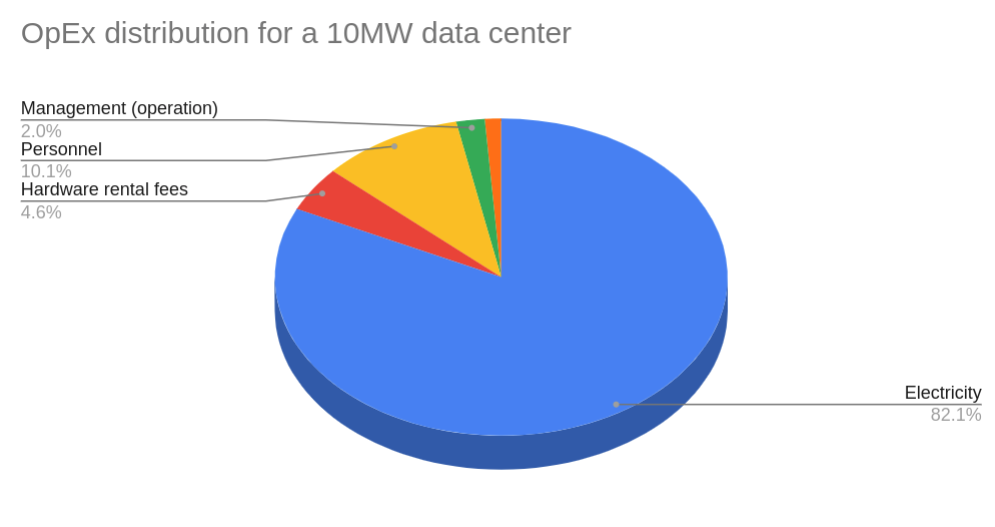
\includegraphics[width=0.7\textwidth]{opexdistribution10mw}
    \label{figure:opexdistribution10mw}
\end{figure}

Zusammenfassend kann festgestellt werden, dass die \ac{OpEx} sich bei einer Mining Kapazität von 10MW auf circa 317.897 USD
belaufen.\footcite[Vgl.][]{appendix:opex} Nun müssen durch das Mining Einnahmen generiert werden, die diese Ausgaben über
die Zeit hinweg amortisieren, damit das Unternehmen in der Lage ist, Gewinn zu erzielen. Die Verteilung der einzelnen Kosten
ist in Abbildung \ref{figure:opexdistribution10mw} relativ auf jährlicher Basis abgebildet.

Wie bereits in der Auszählung für \ac{CapEx} beschrieben, wird die finanzielle Effektivität eines Mining Gerätes durch
die Größe \RM betrachtet. Allerdings kann diese sehr stark fluktuieren, da dabei Faktoren, wie der Tauschkurs von Bitcoin
in USD (s. Ziffer "`Exchanges"' in Abb. \ref{figure:valuechaindatacenter}) und auch \DP, sich abhängig von den Mining
Parametern, wie Difficulty und Netzwerk Hashrate, entwickeln. Eine genaue Vorhersage ist daher nicht möglich, weshalb dort
mit verschiedenen Szenarien gerechnet wird.\footcite[Vgl.][]{appendix:s19proassumptions} Aus diesen wird dann letztendlich ein
gewichteter Durchschnitt gebildet, welcher für die Kalkulation verwendet wird.\footcite[Vgl.][]{appendix:s19proassumptions}

\begin{figure}[H]
    \caption{Kosten- und Wertflüsse bei einem Mining Rechenzentrum}
    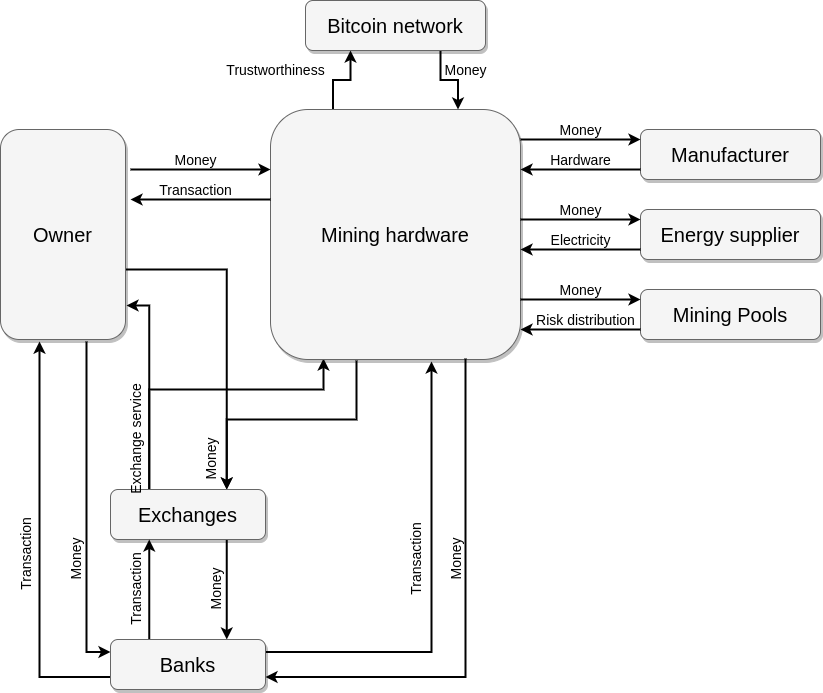
\includegraphics[width=0.7\textwidth]{valuechaindatacenter}
    \label{figure:valuechaindatacenter}
    \\
    \cite[Quelle: In Anlehnung an][Abb. 3]{derks2018chaining}
\end{figure}

Bei dem vorliegenden Beispiel des Mining Datencenters wurden die folgenden Szenarien mit Eintrittswahrscheinlichkeiten gebildet:

\begin{table}[H]
    \caption{Mining Effektivität Szenarien}
    \label{tbl:miningrewardscenario}
    \begin{tabularx}{\textwidth}[ht]{X||X|X|X}
        Szenario & \RM & Eintrittswahrscheinlichkeit & Mining Einnahmen  \\
        \hline\hline
        Worst-Case & $0,07\ USD / \frac{TH}{s} / day$ & $30\%$ & $8.224.610\frac{USD}{Year}$ \\
        \hline
        Most-Probable & $0,09\ USD / \frac{TH}{s} / day$ & $40\%$ & $10.574.499\frac{USD}{Year}$ \\
        \hline
        Optimal & $0,27\ USD / \frac{TH}{s} / day$ & $30\%$ & $31.723.497\frac{USD}{Year}$ \\
    \end{tabularx} \\
    \cite[Quelle: In Anlehnung an][]{appendix:s19proassumptions}
\end{table}

Wie anhand von Tabelle \ref{tbl:miningrewardscenario} erkennbar ist, fluktuieren die Einnahmen zwischen 10 und über
30 Millionen \ac{USD}, was eine beträchtliche Unschärfe darstellt. Daher ist bei diesen Werten eine Optimierung anzustreben.
Ob dies möglich ist, wird in den folgenden Kapiteln evaluiert. Weiterhin werden in diesen Berechnungen keine weiteren
Risiken benannt und daher in der Kalkulation ignoriert. Dies stellt auch eine Möglichkeit der Verbesserung dar,
da mit einer zusätzlichen Risikoanalyse die Eintrittswahrscheinlichkeiten besser abgeschätzt werden können.

Basierend auf allen finanziellen Daten sind der Cashflow und der Break-Even Punkt berechenbar. Das Ergebnis einer
solchen Berechnung findet sich in Abbildung \ref{figure:datacentercashflow}. In der Abbildung sind die jeweiligen Größen
auf einer jährlichen Basis angetragen und zeigen die Entwicklung von \ac{CapEx} und \ac{OpEx} über die Jahre hinweg.

\begin{figure}[H]
    \caption{Cashflow und Break-Even eines Mining Rechenzentrums}
    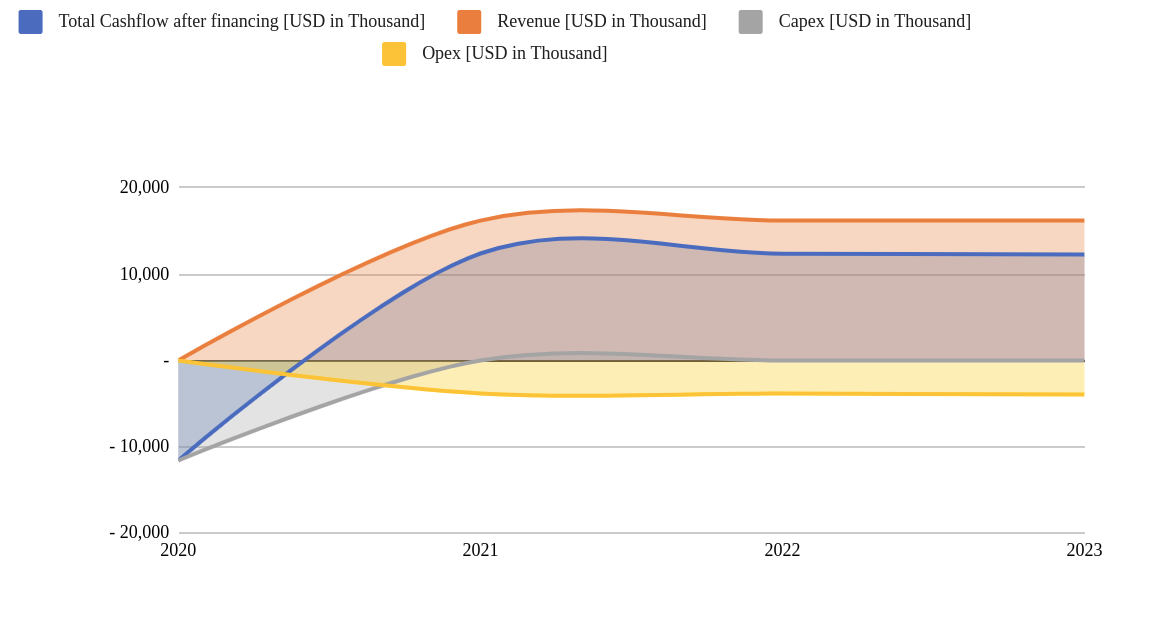
\includegraphics[width=0.7\textwidth]{datacentercashflow}
    \label{figure:datacentercashflow}
    \\
    \cite[Quelle: ][]{appendix:summaryofinvestment}
\end{figure}

Letztendlich gibt es weitere Faktoren, die auf die Effektivität eines Datencenters und damit auf der Seite der
Einnahmen Einfluss nehmen:
\begin{itemize}
    \item \textbf{Klima: }Das Klima wirkt sich auf die Effektivität der Miner aus und bestimmt auch maßgeblich
    die Dimensionierung der Kühlung. Dementsprechend ist es das Ziel bei der Ortswahl eine optimale Kombination aus
    Strompreis, der die \ac{OpEx} maßgeblich bestimmt, und den \ac{CapEx} für die Kühlung, die einen
    großen Anteil ausmacht, zu erreichen. Das genaue Klima wird allerdings nicht in Betrachtungen einbezogen.
    \item \textbf{Versorgungssicherheit: }Dieser Faktor beschreibt die Sicherheit der nötigen externen Infrastruktur,
    wie Internet und Elektrizität. Da jeder Ausfall zwangsläufig in einen effektiven Komplettausfall des Rechenzentrums
    mündet, muss dies in die Betrachtung einbezogen werden.
\end{itemize}
